\documentclass[11pt]{article}
\usepackage[a3paper, landscape, margin=1.8cm]{geometry}
\usepackage{tikz}
\usetikzlibrary{arrows.meta, fit, backgrounds, calc}
\usepackage[T1]{fontenc}
\usepackage{xcolor}
\pagestyle{empty}

\definecolor{CliD}{HTML}{1A6060}
\definecolor{CliF}{HTML}{D4EEEE}
\definecolor{MCD} {HTML}{2C3E7A}
\definecolor{MCF} {HTML}{DDE3F5}
\definecolor{DrmD}{HTML}{7A4010}
\definecolor{DrmF}{HTML}{FAE8D4}
\definecolor{IfcD}{HTML}{5B2080}
\definecolor{IfcF}{HTML}{EEE0FA}
\definecolor{DfiD}{HTML}{0D1F3C}
\definecolor{AW}  {HTML}{1A6060}
\definecolor{AR}  {HTML}{8B4500}
\definecolor{AI}  {HTML}{5B2080}
\definecolor{AG}  {HTML}{444444}

\tikzset{
  BLK/.style args={#1/#2}{
    rectangle, rounded corners=5pt,
    draw=#1, fill=#2, text=#1,
    font=\normalsize\bfseries, align=center,
    inner sep=8pt, minimum width=3.0cm, minimum height=1.1cm,
    line width=1.0pt
  },
  RGN/.style={
    draw=#1, fill=#1!5, rounded corners=10pt,
    dashed, line width=1.2pt
  },
  ARR/.style={
    -{Stealth[length=6pt,width=4.5pt]},
    line width=1.1pt, color=#1
  },
}

\begin{document}
\centering
\vspace*{2pt}
{\LARGE\bfseries\color{DfiD} Reconfigurable DDR Memory Controller}\\[5pt]
{\normalsize\color{gray} Microarchitecture Block Diagram \quad|\quad Rev\,1.0}\\[18pt]

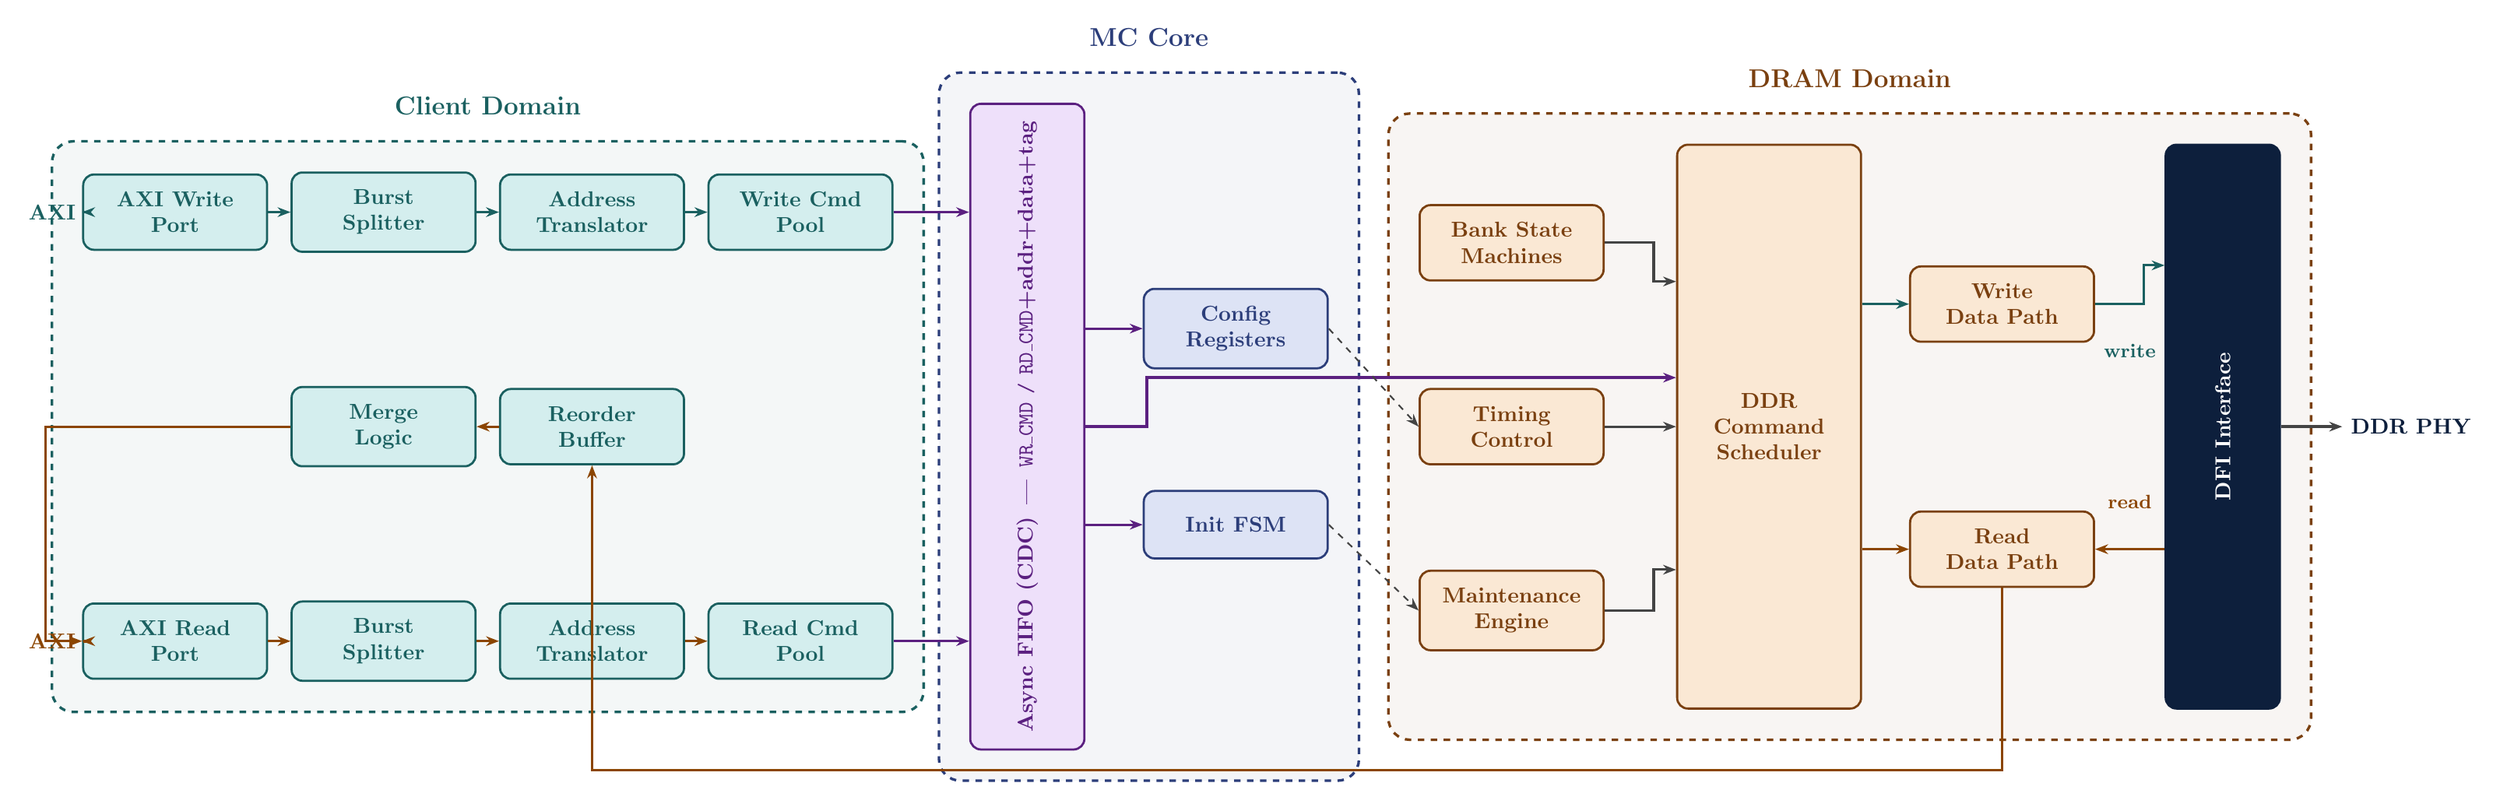
\begin{tikzpicture}[x=1cm,y=1cm,xshift=-1.5cm]

%================ CLIENT DOMAIN =================
\node[BLK=CliD/CliF] (awp)  at (-1.7, 3.5) {AXI Write\\Port};
\node[BLK=CliD/CliF] (bsW)  at ( 1.7, 3.5) {Burst\\Splitter};
\node[BLK=CliD/CliF] (adW)  at ( 5.1, 3.5) {Address\\Translator};
\node[BLK=CliD/CliF] (wcpl) at ( 8.5, 3.5) {Write Cmd\\Pool};

\node[BLK=CliD/CliF] (arp)  at (-1.7,-3.5) {AXI Read\\Port};
\node[BLK=CliD/CliF] (bsR)  at ( 1.7,-3.5) {Burst\\Splitter};
\node[BLK=CliD/CliF] (adR)  at ( 5.1,-3.5) {Address\\Translator};
\node[BLK=CliD/CliF] (rcpl) at ( 8.5,-3.5){Read Cmd\\Pool};

\node[BLK=CliD/CliF] (rrb)  at (5.1,0) {Reorder\\Buffer};
\node[BLK=CliD/CliF] (mlg)  at (1.7,0) {Merge\\Logic};

%================ MC CORE =================
\node[BLK=IfcD/IfcF,
minimum width=1.6cm,minimum height=9.2cm,text width=1.3cm]
(cdc) at (12.2,0)
{\rotatebox{90}{Async FIFO (CDC)\enspace|\enspace
\texttt{WR\_CMD / RD\_CMD}+addr+data+tag}};

\node[BLK=MCD/MCF] (cfg)  at (15.6,1.6) {Config\\Registers};
\node[BLK=MCD/MCF] (init) at (15.6,-1.6) {Init FSM};

%================ DRAM DOMAIN =================
\node[BLK=DrmD/DrmF] (bfsm)  at (20.1,3.0) {Bank State\\Machines};
\node[BLK=DrmD/DrmF] (tctl)  at (20.1,0.0) {Timing\\Control};
\node[BLK=DrmD/DrmF] (maint) at (20.1,-3.0){Maintenance\\Engine};

\node[BLK=DrmD/DrmF,
minimum width=3cm,minimum height=9.2cm]
(sched) at (24.3,0) {DDR\\Command\\Scheduler};

\node[BLK=DrmD/DrmF] (wdp) at (28.1,2.0) {Write\\Data Path};
\node[BLK=DrmD/DrmF] (rdp) at (28.1,-2.0){Read\\Data Path};

\node[BLK=DfiD/DfiD,
minimum width=1.6cm,minimum height=9.2cm,
text=white,text width=1.3cm]
(dfi) at (31.7,0)
{\rotatebox{90}{\bfseries DFI Interface}};

%================ REGION BOXES =================
\begin{scope}[on background layer]
\node[RGN=CliD,
fit=(awp)(bsW)(adW)(wcpl)(arp)(bsR)(adR)(rcpl)(rrb)(mlg),
inner sep=14pt] (crgn) {};

\node[RGN=MCD,
fit=(cdc)(cfg)(init),
inner sep=14pt] (mrgn) {};

\node[RGN=DrmD,
fit=(bfsm)(tctl)(maint)(sched)(wdp)(rdp)(dfi),
inner sep=14pt] (drgn) {};
\end{scope}

\node[font=\large\bfseries,color=CliD,above=8pt] at (crgn.north) {Client Domain};
\node[font=\large\bfseries,color=MCD, above=8pt] at (mrgn.north) {MC Core};
\node[font=\large\bfseries,color=DrmD,above=8pt] at (drgn.north) {DRAM Domain};

%================ AXI INPUTS =================
\draw[ARR=AW,line width=1.3pt] (-3.2,3.5)--(awp.west);
\draw[ARR=AR,line width=1.3pt] (-3.2,-3.5)--(arp.west);

\node[left,font=\normalsize\bfseries,color=AW] at (-3.2,3.5) {AXI};
\node[left,font=\normalsize\bfseries,color=AR] at (-3.2,-3.5){AXI};

%================ CLIENT PIPELINES =================
\draw[ARR=AW] (awp.east)--(bsW.west);
\draw[ARR=AW] (bsW.east)--(adW.west);
\draw[ARR=AW] (adW.east)--(wcpl.west);

\draw[ARR=AR] (arp.east)--(bsR.west);
\draw[ARR=AR] (bsR.east)--(adR.west);
\draw[ARR=AR] (adR.east)--(rcpl.west);

%================ CDC INPUTS =================
\draw[ARR=AI] (wcpl.east)--(cdc.west|-wcpl.east);
\draw[ARR=AI] (rcpl.east)--(cdc.west|-rcpl.east);

\draw[ARR=AI] (cdc.east|-cfg)--(cfg.west);
\draw[ARR=AI] (cdc.east|-init)--(init.west);

\draw[ARR=AI,line width=1.4pt]
(cdc.east|-tctl)--++(1,0)--++(0,0.8)--(sched.west|-{(0,0.8)});

%================ CONTROL PATHS =================
\draw[ARR=AG,dashed,line width=0.75pt]
(cfg.east) -- (tctl.west);

\draw[ARR=AG,dashed,line width=0.75pt]
(init.east) -- (maint.west);

%================ SCHEDULER INPUTS =================
\draw[ARR=AG] (bfsm.east)--++(0.8,0)|-(sched.west|-bfsm.south);
\draw[ARR=AG] (tctl.east)--(sched.west);
\draw[ARR=AG] (maint.east)--++(0.8,0)|-(sched.west|-maint.north);

%================ DATA PATHS =================
\draw[ARR=AW] (sched.east|-wdp)--(wdp.west);
\draw[ARR=AR] (sched.east|-rdp)--(rdp.west);

\draw[ARR=AW]
(wdp.east)--++(0.8,0)|-(dfi.west|-wdp.north);

\node[above,font=\small\bfseries,color=AW]
at ($(wdp.east)!0.5!(dfi.west)$){write};

\draw[ARR=AR]
(dfi.west|-rdp.center)--(rdp.east);

\node[below,font=\small\bfseries,color=AR]
at ($(dfi.west)!0.5!(rdp.east)$){read};

%================ READ RETURN =================
\draw[ARR=AR]
(rdp.south)
-- (rdp.south |- 0,-5.6)
-- (rrb.south |- 0,-5.6)
-- (rrb.south);

\draw[ARR=AR] (rrb.west)--(mlg.east);

\draw[ARR=AR]
  (mlg.west) -- ++(-4.0,0)
  -- ++(0,-3.5)
  -- (arp.west);

%================ DDR PHY =================
\draw[ARR=AG,line width=1.5pt]
(dfi.east)--++(1,0)
node[right,font=\normalsize\bfseries,color=DfiD]{DDR PHY};

\end{tikzpicture}
\end{document}